\documentclass[UTF8]{ctexart}

\usepackage[a4paper, left=3.17cm, right=3.17cm, top=2.54cm, bottom=2.54cm]{geometry}
\usepackage[T1]{fontenc}
\usepackage{mathptmx}
\usepackage{amsmath}
\usepackage{amsfonts}
\usepackage{chemformula}
\usepackage{cite}
\usepackage[colorlinks, linkcolor=black, anchorcolor=black, citecolor=black]{hyperref}
\usepackage{graphicx}
\usepackage{fancyhdr}
\usepackage{enumitem}
\usepackage{listings}

\setlength{\parskip}{0.5em}
\title{\heiti 面向对象程序设计\ \ 大程报告}
\author{\Large \kaishu \textup{刘泓健\ \ 吴一航}}

\ctexset {
    section = {
        format={\Large \bfseries \heiti} 
        } 
    }

\lstset{
    columns=fixed,       
    numbers=left,                                        % 在左侧显示行号
    numberstyle=\tiny\color{gray},                       % 设定行号格式
    frame=none,                                          % 不显示背景边框
    backgroundcolor=\color[RGB]{245,245,244},            % 设定背景颜色
    keywordstyle=\color[RGB]{40,40,255},                 % 设定关键字颜色
    numberstyle=\tiny,keywordstyle=\color{blue!70},
    commentstyle=\color{red!50!green!50!blue!50},frame=shadowbox,
    rulesepcolor=\color{red!20!green!20!blue!20},basicstyle=\ttfamily,
    stringstyle=\rmfamily\slshape\color[RGB]{128,0,0},   % 设置字符串格式
    showstringspaces=false,                              % 不显示字符串中的空格
    language=C++,                                        % 设置语言
    }

\pagestyle{fancy}
\fancyhf{}
\cfoot{\thepage}
\fancyhead[C]{面向对象程序设计\ \ 大程报告}
\begin{document}

\begin{titlepage}
	\newcommand{\HRule}{\rule{\linewidth}{0.5mm}}
	\begin{figure}
        \flushleft
        
\includegraphics[scale=0.4]{0.png}
    \end{figure}
    \center 
	\quad\\[1.5cm]
	\textsl{\Large Zhejiang University }\\[0.5cm] 
	\textsl{\large College of Computer Science and Technology}\\[0.5cm] 
	\makeatletter
	\HRule \\[0.4cm]
	{ \huge \bfseries \@title}\\[0.4cm] 
	\HRule \\[1.5cm]
	\begin{minipage}{0.4\textwidth}
		\begin{flushleft} \Large
			\emph{Author:}\\
			\@author 
		\end{flushleft}
	\end{minipage}
	~
	\begin{minipage}{0.4\textwidth}
		\begin{flushright} \Large \kaishu
			\emph{Supervisor:} \\
			\textup{翁恺}
		\end{flushright}
	\end{minipage}\\[3cm]
	\makeatother
	{\large An Assignment submitted for the ZJU:}\\[0.5cm]
	{\large {211C0010\ \ 面向对象程序设计}}\\[0.5cm]
	{\large \today}\\[2cm] 
	\vfill 
\end{titlepage}
    
    \section{大程简介}
    在课程大程中,我们实现了一个完整的MUD游戏。这一游戏的主题灵感来源于FiraxisGames的著名游戏《文明》系列,
    希望实现的是游戏主人公从山洞中走出直到统治文明的过程。
    虽然本项目的初衷是完成本学期oop的课程大程,但是我们的目标不止于此。
    我们的设计具有强大的可拓展性,实际上,用户只需要修改数据文件即可实现游戏的再生产。
    本项目开源地址为https://github.com/FrightenedFoxCN/OOP\_capolization, 
    对于本项目实现的基本框架感兴趣可以使用,完善,或者添加自己希望实现的功能。

    \section{使用的技术}
    \begin{enumerate}
        \item 基于C++的面向对象编程技术
        
        在这一大程中,我们基于C++开发,通过几个主要类的设计进行组织,
        使用了命名空间、虚函数、异常处理、流等C++编程技术。一方面将课程所学知识
        应用于我们的设计,另一方面也通过网络等途径在编程过程中学习新的特性。
        \item 基于Git的版本管理
        
        我们的项目目前已在GitHub上开源,开发过程中也一直使用git的方式进行版本管理。
        \item 基于JSON的数据管理
        
        对于这一点,我们需要说明的是,在我们代码的lib文件夹中,引入了一个
        JSON parser库便于处理我们的JSON数据。我们JSON文件的处理方式在一定
        程度上参考了人生重开模拟器的组织方式。这一设计相对于使用其他
        文件组织方式更为简便、清晰。
    \end{enumerate}

    \section{项目特色}
    \begin{enumerate}
        \item 可扩展性
        
        这一点已在第一部分大程简介有所描述,此处不再赘述。
        \item 实现了游戏存档功能
        
        这一实现基于我们的使用JSON的数据处理方式,这使得我们能够以很
        便捷易懂的方式完成游戏存档与重新读入数据的操作。

        \item 完整的测试代码
        
        我们不仅实现了最后的release版本,在开发过程中,我们对于每一个模块,例如
        character类、dialog类以及我们的JSON数据处理,都做了基本的测试。详细的
        测试代码在testbench文件夹中。

        \item 清晰的开发流程,文件框架,以及代码规范。这一部分在doc文档的general.md
        中有所说明。

        \item 故事设计埋藏深意(或许需要进行很多次游戏遍历大量分支才能有所体会)。
    \end{enumerate}

    \section{代码基本框架}
\begin{lstlisting}
.
|——assets(游戏所需图片、文案等资源)
     |——dialog.json
|——doc(大程文档,如规范性文档以及注释文档等)
     |——general.md(规范文档)
|——include(自主设计的头文件)
     |——character.h
     |——dialog.h
|——lib(外部引用库,如JSON parser及图形界面等所需外部库)
     |——nlohmann
          |——...
|——src(大程源代码)
     |——core
          |——dialog.cpp
          |——character.cpp
     |——utils
     |——main.cpp(初始执行文件)
     |——Makefile
|——testbench(测试文件)
     |——xcharacter.cpp
     |——xjson.cpp
     |——xdialog.cpp
     |——xjsonfile.cpp
|——Makefile
\end{lstlisting}
    
    \section{基本设计}
    我们的程序入口为main函数,在进行了一系列初始化,创建新文件或者从文件中
    读入文件。接下来我们开始游戏。实际上main中的整体流程是并不复杂的,
    实际上就是通过调用Dialog中的函数得到下一次的分支,然后通过解析出
    JSON中的内容调用构造函数构造出这个dialog对象,如此往复,直到结局。

    在对话类的设计中,我们关注以下几个重要的属性:
    \begin{enumerate}
        \item branch:分支,根据玩家所作出的选择进入某一分支
        \item randBranch:随机分支,玩家无需做出选择,系统自动根据概率计算创造随机分支
        \item condBranch:条件分支,根据所给条件决定分支(实际上与角色的属性有关)
        \item nextDialog:指向下一dialog的信息
    \end{enumerate}
    
    在角色Character类的设计中,我们主要实现的是几个属性,以及如何将这些属性
    保存进JSON文件/从JSON中读入。以及如何将我们在进入一定分支后,对角色自身
    属性产生一定的的影响。

    在整体设计中,我们设计了四个死亡结局,剩余一个可以苟活的结局。
    对话作者在其中设计了洛夫克拉夫特式的结局,蕴含深意,与我们选择的主题契合。
    我们程序执行流程图见assets/story_p1.md。

    \section{运行与使用方式}
    运行在windows环境下需要mingw32-make release即可,Linux环境使用make命令进行
    make release也可以。接下来./test即可开始游戏。

    进入游戏后,首先输入用户名,新用户新建用户名即可。接下来开始游戏,当需要输入时,
    根据显示输入即可,如果输入q则会退出并存档。注意,由于游戏中有很多的随机branch,
    所以运气不好可能会陷入循环,或者很快就会落入死亡结局。
    
    如果遇到编码问题,请将终端中的字符设置为UTF-8格式。

    \section{运行结果展示}
    \begin{figure}[h]
        \centering
        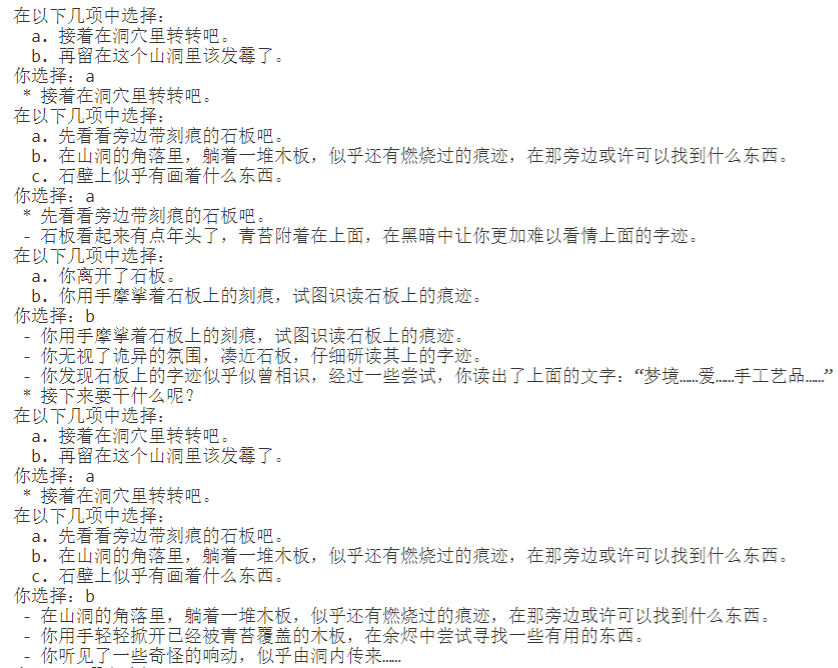
\includegraphics[scale=0.45]{1.png}
    \end{figure}

    \section{一些展望}
    虽然本次大程到目前告一段落,但是我们对于这一游戏的设计还没有结束。
    我们一方面希望能给这个游戏一个更加圆满的设计,当然限于时间和灵感,
    我们目前的设计还有可以扩展的空间。另一方面,我们希望将这一框架
    实现为一个能够便捷开发所有具有类似设计思路的MUD游戏的基本框架,
    我们还可以实现将一定格式的流程图转直接转化为JSON文件,使得开发更为便捷。
    除此之外,我们还可以对存档文件做加密,这一点更加接近真实情况,也防止后门。

\end{document}